%% thesis.tex 2014/04/11
%
% Based on sample files of unknown authorship.
%
% The Current Maintainer of this work is Paul Vojta.

\documentclass[masters]{ucbthesis}

\usepackage{biblatex}
\usepackage{rotating} % provides sidewaystable and sidewaysfigure

\usepackage[utf8]{inputenc}
\usepackage{amsmath,amsthm,amssymb}

\usepackage{mathtools}
\usepackage{bbm}
\usepackage{marvosym}
\usepackage[hidelinks]{hyperref}
\usepackage{framed}
\usepackage{enumitem}
\usepackage{float}
\usepackage{bm}
\usepackage{tabularx}
\usepackage{booktabs}
\usepackage{url}


\newtheorem{theorem}{Theorem}[chapter]
\newtheorem{proposition}[theorem]{Proposition}
\newtheorem{lemma}[theorem]{Lemma}
\newtheorem{corollary}[theorem]{Corollary}
\newtheorem{conjecture}[theorem]{Conjecture}
\newtheorem{postulate}[theorem]{Postulate}
\theoremstyle{definition}
\newtheorem{definition}[theorem]{Definition}
\newtheorem{example}[theorem]{Example}
\newtheorem{observation}{Observation}
\newtheorem{remark}[theorem]{Remark}

\newcommand{\vertiii}[1]{{\left\vert\kern-0.25ex\left\vert\kern-0.25ex\left\vert#1 
    \right\vert\kern-0.25ex\right\vert\kern-0.25ex\right\vert}}

\newcommand*\enlarg[2]{\bar{#1}_{#2}}
\newcommand*\cohnorm[1]{\vertiii{#1}^{\mathrm{coh}}_{K,\varphi,\alpha,\gamma}}

% To compile this file, run "latex thesis", then "biber thesis"
% (or "bibtex thesis", if the output from latex asks for that instead),
% and then "latex thesis" (without the quotes in each case).

% Double spacing, if you want it.  Do not use for the final copy.
% \def\dsp{\def\baselinestretch{2.0}\large\normalsize}
% \dsp

% If the Grad. Division insists that the first paragraph of a section
% be indented (like the others), then include this line:
% \usepackage{indentfirst}

\addtolength{\abovecaptionskip}{\baselineskip}

\bibliography{references}

\hyphenation{mar-gin-al-ia}
\hyphenation{bra-va-do}

\begin{document}

% Declarations for Front Matter

\title{Chipsplitting Games: A Combinatorial Approach to Classifying One-Dimensional Discrete Statistical Models with Rational Maximum Likelihood Estimator}
\author{Viet-Duc Nguyen}
\degreesemester{Winter}
\degreeyear{2024}
\degree{Master of Science}
\chair{Professor Carlos Améndola}
\othermembers{Professor Christian Haase}
% For a co-chair who is subordinate to the \chair listed above
% \cochair{Professor Benedict Francis Pope}
% For two co-chairs of equal standing (do not use \chair with this one)
% \cochairs{Professor Richard Francis Sony}{Professor Benedict Francis Pope}
\numberofmembers{3}
% Previous degrees are no longer to be listed on the title page.
% \prevdegrees{B.A. (University of Northern South Dakota at Hoople) 1978 \\
%   M.S. (Ed's School of Quantum Mechanics and Muffler Repair) 1989}
\field{Mathematics}
% Designated Emphasis -- this is optional, and rare
% \emphasis{Colloidal Telemetry}
% This is optional, and rare
% \jointinstitution{University of Western Maryland}
% This is optional (default is Berkeley)
% \campus{Berkeley}

% For a masters thesis, replace the above \documentclass line with
% \documentclass[masters]{ucbthesis}
% This affects the title and approval pages, which by default calls this
% document a "dissertation", not a "thesis".

\maketitle
% Delete (or comment out) the \approvalpage line for the final version.
% \approvalpage
\copyrightpage

\begin{alwayssingle}
\pagenumbering{gobble}
\section*{Zusammenfassung in deutscher Sprache}

Die vorliegende Ausarbeitung setzt die Forschung von Arthur Bik und Orlando Marigliano zur Klassifizierung ein-dimensionaler diskreter statistischer Modelle mit rationalen Maximum Likelihood Schätzern unter Verwendung fundamentaler Modelle fort. Wir erzielen bedeutende Fortschritte beim Beweis zur endlichen Anzahl der fundamentalen Modelle im Wahrscheinlichkeitssimplex \( \Delta_5 \). Zudem bestimmen wir die Anzahl der fundamentalen Modelle im Simplex \( \Delta_6 \) mit einem maximalen Grad von 11.

\end{alwayssingle}

% (This file is included by thesis.tex; you do not latex it by itself.)

\begin{abstract}

% The text of the abstract goes here.  If you need to use a \section
% command you will need to use \section*, \subsection*, etc. so that
% you don't get any numbering.  You probably won't be using any of
% these commands in the abstract anyway.


This paper continues the research of Arthur Bik and Orlando Marigliano on the classification of one-dimensional discrete statistical models with rational maximum likelihood estimators using fundamental models. We determine the number of fundamental models in the simplex \( \Delta_6 \) with a maximum degree of eleven, a result that was previously unknown. Moreover, we reduce the number of cases to consider for proving the finite number of fundamental models in the simplex \( \Delta_6 \) with a maximum degree of eleven from 300,000 to 12,000, making a proof far more feasible in the future. The algorithm underpinning these key results is embedded in the framework of solving non-trivial hyperfield linear systems, which we have developed specifically for this thesis. All the code is publicly available on GitHub.


\end{abstract}


\begin{frontmatter}

% You can delete the \clearpage lines if you don't want these to start on
% separate pages.

\tableofcontents
\clearpage
%\listoffigures
%\clearpage
%\listoftables


\end{frontmatter}

\pagestyle{headings}

% (Optional) \part{First Part}
\pagenumbering{arabic}

\chapter{Introduction} 

In statistics, we come across various collections of probability distributions, such as the normal distribution, Poisson distribution, and binomial distribution. These distributions are used to model random variables in applications and are referred to as \emph{statistical models}. Precisely, a statistical model is just a set of probability distributions. If the set contains only discrete distributions, we call it a \emph{discrete statistical model}. In this case, discrete statistical models are just subsets of the probability simplex \( \Delta_n \coloneqq \left\{ p \in \mathbb{R}^{n + 1} \mid \sum p_i = 1 \right\} \). 

A discrete distribution \( p \in \mathcal{M} \subset \Delta_n \) from a discrete statistical model encapsulates the probabilities of observing the states \( 0, \dots, n \), i.e. if \( X \in \left\{ 0, \dots, n \right\} \) is a discrete random variable, then the state \( X = i \) occurs with probability \( p_i \) for all \( i = 0, \dots, n \). Say we have a binomial random variable \( X \) with \( n + 1 \) states, then \( p_i = \binom{n}{i} \theta^i (1-\theta)^{n-i} \) computes the probability of observing \( i \) successes in \( n \) trials with success probability \( \theta \in [0,1] \). The set \( \mathcal{M} \) of all probability distributions of that form, i.e. \( \mathcal{M} = \left\{ (\binom{n}{i} \theta^i (1-\theta)^{n-i})_{i=0}^n \mid \theta \in [0,1] \right\} \), is our first example of a discrete statistical model, and is known as the \emph{binomial model}.

\begin{figure}
    \centering
    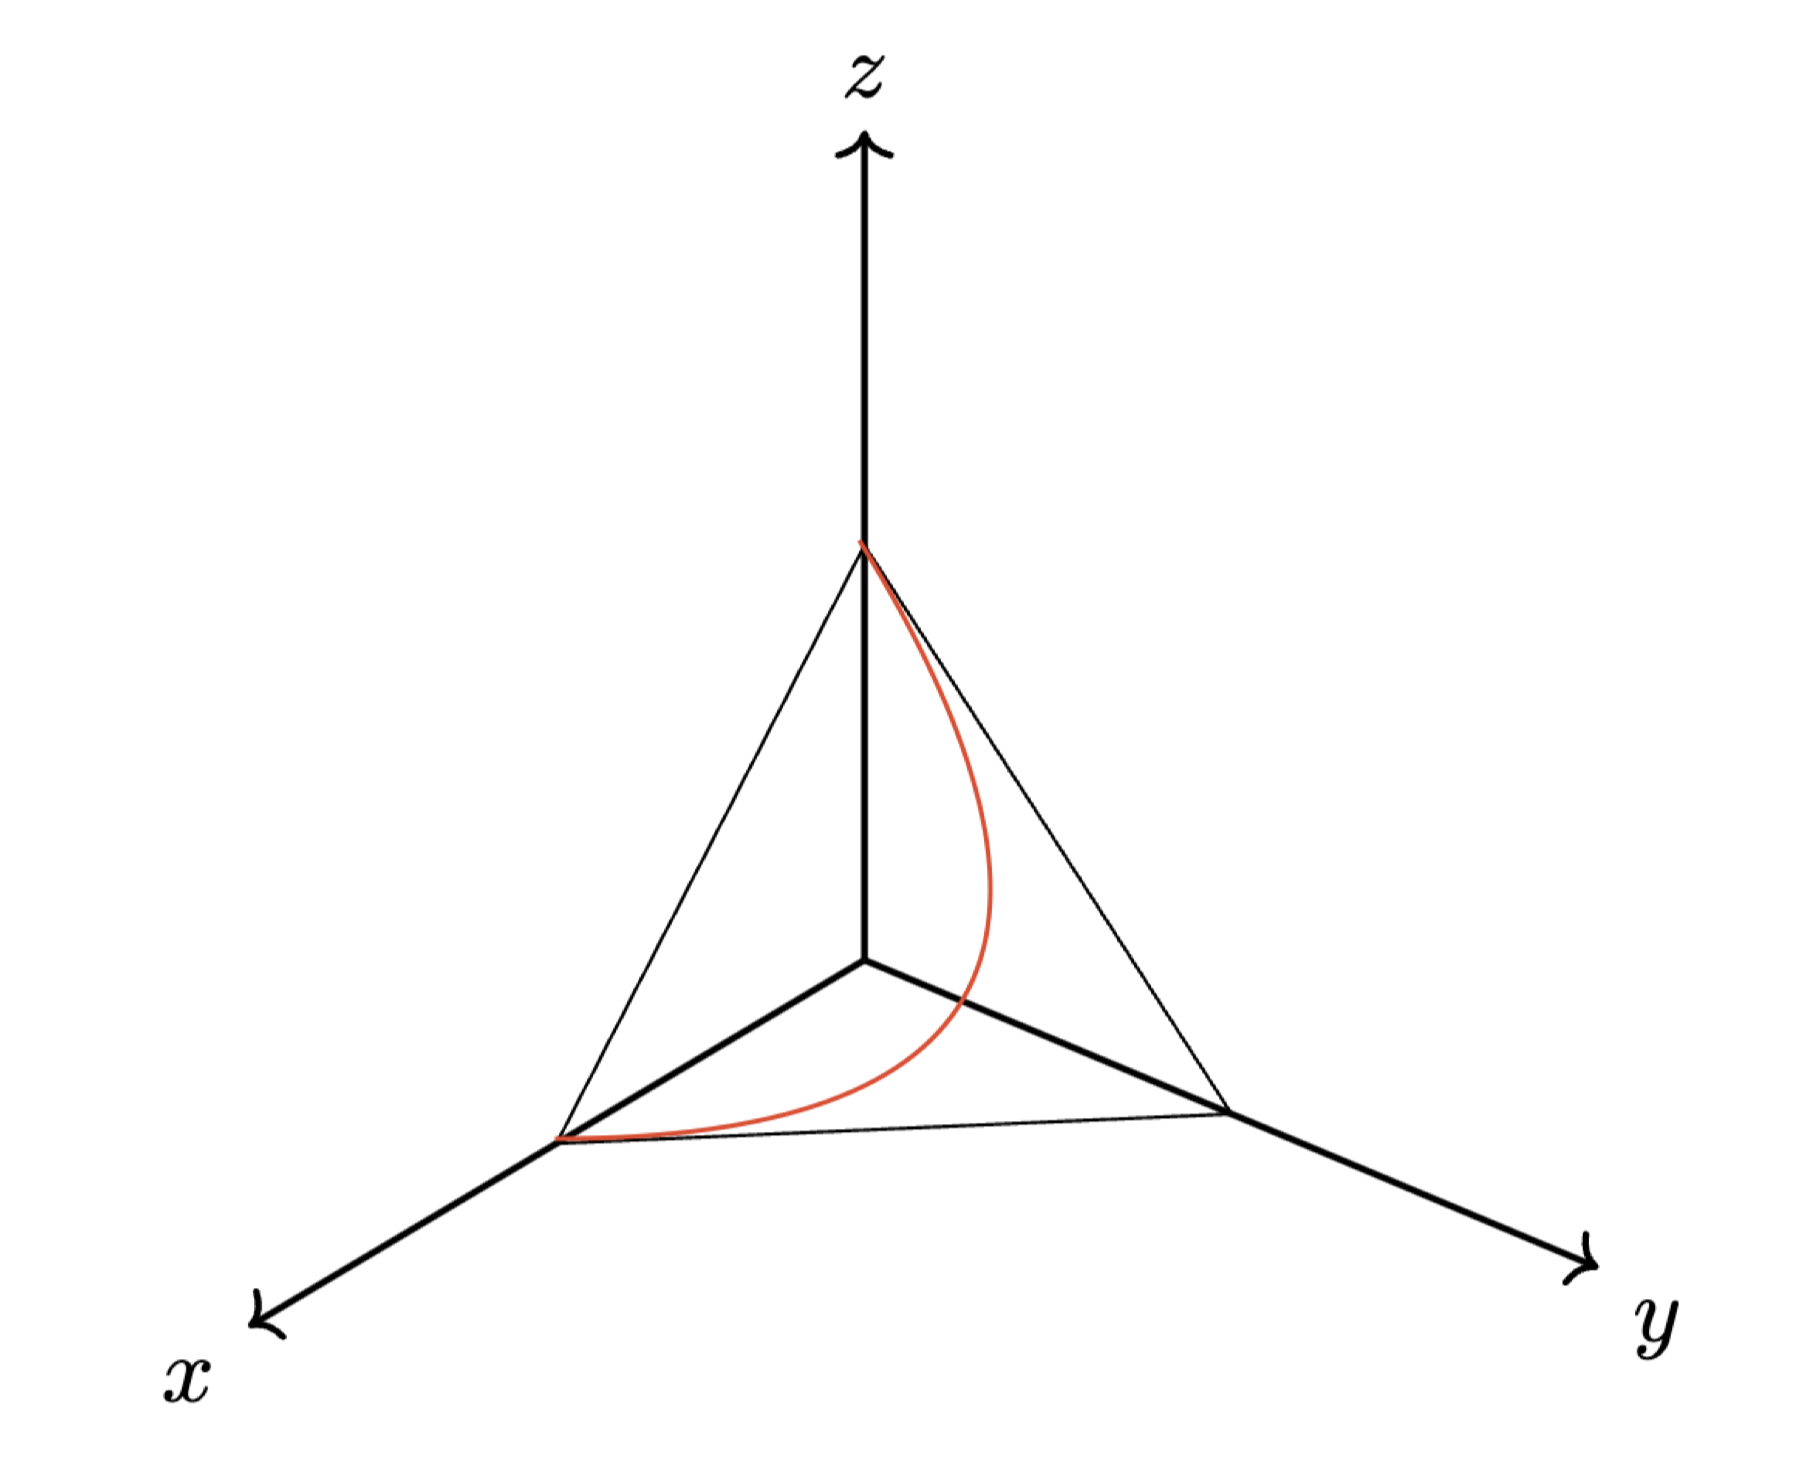
\includegraphics[width=0.4\textwidth]{assets/binom-discrete-model.png}
    \caption{This figure shows the probability simplex \( \Delta_2 \) with the binomial model (red curve). Every point on the curve is a binomial distribution.}
    \label{fig:binom-discrete-model}
\end{figure}

Given a statistical model \( \mathcal{M} \subset \Delta_n \) and data \( u \in \mathbb{N}^{n+1} \), a typical problem in statistics is to find a distribution from a statistical model that best describes the data. ``Best'' can mean a lot of things, but in \emph{maximum likelihood estimation} it means finding the distribution that maximizes the probability of observing the data; the map \( \Phi: \Delta_n \to \mathcal{M}, u \mapsto \hat p \) that assigns the data \( u \) to a distribution \( \hat p \in \mathcal{M}\) from the statistical model is called the \emph{maximum likelihood estimator (MLE)}. This map is characterized by the property that \( \hat p \) maximizes the log-likelihood function \( \ell(p) = \sum u_i \log p_i \) for all \( p \in \mathcal{M} \). 

We focus on \textbf{{one-dimensional {discrete} {statistical} {models} with rational MLE}}. These are models \( \mathcal{M} \) satisfying 
\begin{itemize}
    \item \( \mathcal{M} = \mathrm{image}(p) \) for some rational map \( p = (p_0, \dots, p_n): I \to \Delta_n \) where \( p_i \) is rational, \( I \subset \mathbb{R} \) is a union of closed intervals and  \( p(\partial I) \subset \partial \Delta_n \),
    \item all the \( n+1 \) coordinates of the maximum likelihood estimator \( \Phi \) are rational functions in the data \( u \).
\end{itemize}
There are two intriguing questions to ask about statistical models with rational MLE: the first one is about which \emph{form} they take; the second one is more concerned with the \emph{classification} of the statistical models, i.e. can we divide these models into easier to understand classes? An answer to the first question was given by June Huh. He showed that if \( \Phi \) is rational, then each of its coordinates is an alternating product of linear forms with a numerator and denominator of the same degree, see \cite{huh2013varieties, huh2013maximum, duarte2021discrete}. For the second question, Arthur Bik and Orlando Marigliano classified all one-dimensional discrete statistical models with rational MLE using \emph{fundamental models} \cite{bik2022classifying}.

This thesis continues the work of Bik and Marigliano. In the first half, we present their classification results on how fundamental models serve as the building blocks of one-dimensional discrete models with rational MLE. In the second half, we establish and extend their finding that there are only finitely many fundamental models within the probability simplices \( \Delta_n  \) for \( n \leq 4 \). Due to the complexity of the problem, the cases \( n \geq 5 \) were left open. We make progress for \( n = 5 \) by reducing the number of cases to check from 300,000 to 12,000. Additionally, this thesis introduces new results on the number of fundamental models in \( \Delta_6 \), with a maximum degree of eleven, and provides an algorithm for solving non-trivial hyperfield linear systems, which is essential to all the computational work presented.

The outline of this thesis is as follows: 
\begin{itemize}
    \item Chapter 2 provides a classification of statistical models using fundamental models.
    \item Chapter 3 introduces chipsplitting games and establishes the connection to fundamental models via chipsplitting outcomes.
    \item Chapter 4 develops the \emph{Invertibility Criterion}, and Chapter 5 applies it.
    \item Chapter 6 introduces the \emph{Hyperfield Criterion}, and Chapter 7 uses these tools to establish a bound on the degree for positive support size four outcomes.
    \item Chapter 8 introduces the final tool, the Hexagon Criterion, to tackle outcomes with positive support size five, and Chapter 9 applies it.
    \item Chapter 10 presents new techniques to reduce the number of cases that need to be analyzed to prove that the degree of valid outcomes with support size six is bounded.
    \item Chapter 11 computes the number of fundamental outcomes.
    \item Chapter 12 concludes with a discussion on future research directions and the implications of the findings.
\end{itemize}


The source code for the computations discussed in this thesis is available at \cite{ducrepo}.

\chapter{Classification with Fundamental Models}

In this chapter, we present the classification of one-dimensional discrete statistical models with a rational maximum likelihood estimator (MLE) using fundamental models. The classification is due to Arthur Bik and Orlando Marigliano~\cite{bik2022classifying}. 

\begin{center}
    \textbf{Problem statement:} Can we find a class of easy to understand models that serve as building blocks for all one-dimensional discrete statistical models with rational MLE?
\end{center}
The answer to this question are \emph{reduced} and \emph{fundamental models}.

\section{Parametrization}

It turns out that one-dimensional discrete statistical models with rational MLE admit the following parametrization.

\begin{proposition}\label{prop:parametrization}
    Let \( \mathcal{M} \) be a one-dimensional discrete statistical models with rational maximum likelihood estimator. Then, there exists a map of the form
    \begin{gather*}
        p: [0,1] \to \Delta_n, \quad \theta \mapsto (w_k \theta^{i_k} (1-\theta)^{j_k})_{k=0}^n \\
        i_k, j_k \in \mathbb{Z}_{\geq 0}, \;  w_k \in \mathbb{R}_{> 0} \quad \forall k = 0, \dots, n
    \end{gather*}
    such that \( \mathcal{M} = \mathrm{image}(p) \).
\end{proposition}

We introduce some notation to simplify the proof of Proposition \ref{prop:parametrization}.
Let \( \mathcal{M} \subset \Delta_n \) be a one-dimensional discrete statistical model parametrized by rational functions \( p_0 =  \frac{g_0}{h_0}, \dots, p_n =  \frac{g_n}{h_n} \). Define \( b \) to be the least common multiple of \( h_0, \dots, h_n \) and \( a_i \coloneqq b p_i \). Since \( \sum p_k = 1 \), we can multiply by \( b \) to obtain \( \sum a_k = b \). We see that the polynomials \( a_0, \dots, a_n, b \) determine the statistical model \( \mathcal{M} \), and have no common factors. The log-likelihood function is then given by
\( \ell(p) = \sum u_i \log p_i = \sum u_i \log \frac{a_i}{b} = \sum u_i \log a_i - \sum u_i \log b \).

To find the maximum likelihood estimator, we need find all critical points of the log-likelihood function. This is equivalent to finding the roots of the gradient of the log-likelihood function
\begin{align}\label{eq:score-equations}
    \ell(p(\theta))' &= \sum u_k \frac{a_k'}{a_k} - \sum u_k \frac{b'}{b} = 0.
\end{align}
These equations are called the \emph{score equations} in algebraic statistics, and the number of complex solutions to these equations for general data \( u \in \mathbb{C}^{n + 1} \) is called the \emph{maximum likelihood degree} of the statistical model. This ML degree has an important meaning in algebraic statistics, as it is an algebraic measure of the complexity of the maximum likelihood estimation of the model, see \cite{amendola2019maximum, catanese2006maximum, sullivant2023algebraic}.

We have the following relationship between the ML estimator and the ML degree.

\begin{proposition}\label{prop:rational-mle}
    Having rational maximum likelihood estimator can be expressed equivalently by saying that the maximum likelihood degree of the statistical model is one.
\end{proposition}

\begin{proof}
   Refer to \cite{duarte2021discrete} for a proof.
\end{proof}

To prove Proposition \ref{prop:parametrization}, we need the following lemma.

\begin{lemma}\label{lem:two-complex-factors}
    If \( \mathcal{M} \) has rational MLE, then there are exactly two distinct complex linear factors in \( a_0, \dots, a_n \), and \( b \).
\end{lemma}

\begin{proof}
    We prove the lemma in three steps:
    \begin{itemize}
        \item Let \( f \) be the product of all distinct complex linear factors in \( a_0, \dots, a_n, b \).  If we multiply the score equations \eqref{eq:score-equations} by \( f \), we get \( f \cdot \ell(p(\theta))' = \sum u_k f \frac{a_k'}{a_k} - \sum u_k f \frac{b'}{b} = 0 \).
        Note that every linear factor of \( a_k \) with multiplicity \( m \) occurs in \( a_k' \) with multiplicity \( m-1 \); thus every summand of \( \frac{a_k'}{a_k} \) is of the form \( \frac{\lambda}{(x-\xi)} \), where \( \lambda \in \mathbb{R} \) and \( x-\xi \) is some linear factor of \( a_k \); hence \( f \cdot  \frac{\lambda}{(x-\xi)}  \) is of degree \( \mathrm{deg}(f) - 1\), and therefore \( f \cdot \ell(p(\theta))' \) is of degree \( \mathrm{deg}(f) - 1\).

        \item We claim that the roots of \( \ell(p(\theta))' \) are the same as the roots of \( f \cdot \ell(p(\theta))' \). Assume we have shown this claim.  By Proposition \ref{prop:rational-mle} the ML degree is one. So, \( \ell(p(\theta))' \) has one root. Thus, \( f \cdot \ell(p(\theta))' \) has one root, and therefore \( f \cdot \ell(p(\theta))' \) is of degree one. This implies that \( \mathrm{deg}(f) = 2 \) with the previous step. Thus, there are exactly two distinct complex linear factors in \( a_0, \dots, a_n \), and \( b \).
        
        \item It remains to show that the roots stay the same. Clearly, every root of \( \ell(p(\theta))' \) is a root of \( f \cdot \ell(p(\theta))' \). Conversely, we want to show that no new roots are introduced when multiplying by \( f \), i.e. roots of \( f \) are not roots of \(  f \cdot \ell(p(\theta))' \). To do so, we rewrite \( f \cdot \ell(p(\theta))' = \sum_{k=0}^n u_k f \frac{a_k'}{a_k} - \sum_{k=0}^n u_k f \frac{b'}{b} = \sum_{k=0}^{n + 1} v_k f \frac{c_k'}{c_k} \)
        with \( v_k \coloneqq u_k, c_k \coloneqq a_k  \) for \( k=0, \dots,n \), and \(  v_{n+1} \coloneqq - \sum_{k=0}^n u_k \), \( c_{n+1} \coloneqq b \).

        Let \( q \) be a complex linear factor of \( f \). We define polynomials \( r_0, \dots, r_{n+1} \) and \( r \) such that \( c_k = q^{l_k}r_k \), \( f = q r \), and \( r_0, \dots, r_{n+1}, r \) do not have \( q \) as a factor. Then, for \(  k = 0, \dots, n+1 \) we have
        \( f \frac{c_k'}{c_k} = q r \cdot \frac{l_k q^{l_k - 1} q'r_k +  q^{l_k}r_k'}{q^{l_k}r_k} = q r\frac{l_k q' }{q} + q r\frac{r_k'}{r_k} \equiv rl_k q' \pmod q \).
        Thus, we obtain \( f \cdot \ell(p(\theta))' \equiv rq'\sum_{k=0}^{n + 1} v_k l_k \equiv rq' \sum_{k=0}^{n } v_k(l_k - l_{n+1}) \pmod q \).
        Note that by definition of \( l_k \), a value of \( l_k = 0 \) means that \( q \) is not a factor of \( c_k \). By definition of \( f \), at least one \( l_k > 0 \). On the other hand, not all \( l_k \) can be positive since \( a_0, \dots, a_n, b \) share no common factors. Hence, not all \( l_k - l_{n+1} = 0 \) vanish. Hence, for generic data \( u \) we assume \( \sum_{k=0}^{n } v_k(l_k - l_{n+1}) \neq 0 \). This with \( q'r \not \equiv 0 \pmod q \) implies that \( q \) is not a complex linear factor of \( f \cdot \ell(p(\theta))' \). We showed that the roots of \( f \) are not roots of \( f \cdot \ell(p(\theta))' \).
    \end{itemize}
\end{proof}

Equipped with the lemma, we can now prove Proposition \ref{prop:parametrization}.

\begin{proof}
    First, we show that \( I \) is a single closed real interval and not a union of closed intervals. For the sake of contradiction assume that \( I = \bigcup_{k} I_k \) is a union of closed disjoint intervals. By definition of \( \mathcal{M} \) we know that \( p(\partial I) \subset \partial \Delta_n \). Thus, there exist \( \theta_1, \theta_2 \in \partial I_0 \) and \( \theta_3, \theta_4 \in \partial I_1 \) with \( p_i(\theta_1) = p_i(\theta_2) =  0 \) and \( p_j(\theta_3) = p_j(\theta_4) = 0 \) for some \( i,j = 0, \dots, n \). Note that \( \theta_1, \theta_2 \) are roots of \( \frac{a_i}{b} \) and  \( \theta_3, \theta_4 \) are roots of \( \frac{a_j}{b} \). By Lemma \ref{lem:two-complex-factors} exactly two distinct complex linear factors occur in \( a_0, \dots, a_n, b \). Hence, \( \theta_3 = \theta_1 \) or \( \theta_3 = \theta_2 \). Contradiction for \( I_0 \) and \( I_1 \) are disjoint.

    The previous argument shows that \( I = [\alpha, \beta ]\) is a real single closed interval. Thus, the roots of \( a_0, \dots, a_n, b \) are real and take values in \( \partial I = \left\{ \alpha, \beta \right\} \). By a suitable parametrization, we can assume without loss of generality that \( I = [0,1] \). We can now write the polynomials \( a_0, \dots, a_n, b \) as \(  a_k(\theta) = w_k \theta^{i_k} (1-\theta)^{j_k} \), \( b(\theta) = w \theta^{i} (1-\theta)^{j} \)
    with \( w_k, w \in \mathbb{R}_{>0} \), and \( i_k, j_k, i, j \in \mathbb{Z}_{\geq 0} \) for all \( k = 0, \dots, n \). Since \( a_0, \dots, a_n, b \) share no common factors, there exists some \( i_k = 0 \) if \( i > 0 \); however this would contradict \(0 < w_k \leq a_0(0) + \dots + a_n(0) = b(0) = 0\). So \( i = 0 \). Similarly, \( j = 0 \). Finally, we divide \( p \) by \( w \) to obtain \( b \equiv 1 \).
\end{proof}

\begin{corollary}
    Any one-dimensional {discrete} {statistical} {models} with rational MLE can be represented by \( (w_k, i_k, j_k)_{k=0}^n \) for \( w_k \in \mathbb{R}_{>0} \) and \( i_k, j_k \in \mathbb{Z}_{\geq 0} \).
\end{corollary}

\begin{definition}
    The degree \( \mathrm{deg}(\mathcal{M}) \) of a one-dimensional discrete statistical models with rational MLE \( \mathcal{M} \) represented by \( (w_k, i_k, j_k)_{k=0}^n \) is defined as \( \mathrm{max}\left\{ i_k + j_k : k = 0, \dots, n \right\} \).
\end{definition}

\begin{remark}\label{rem:equivalent-models}
    We view two models \( (w_k,i_k,j_k)_{k=0}^n \) and \( (w_k',i_k',j_k')_{k=0}^n \) as the same model if they are equal up to a permutation of the coordinates.
\end{remark}

\begin{example}
    The sequence \( ((1,0,2), (2,1,1), (1,2,0)) \) represents the binomial model with two trials. It has degree two. Its parametrization is given by \( \theta \mapsto ((1-\theta)^2, 2\theta(1-\theta),\theta^2) \). See Figure \ref{fig:binom-discrete-model} for a visualization of the binomial model within the probability simplex \( \Delta_2 \). Note that we treat \( ((1,0,2), (2,1,1), (1,2,0)) \), \( ((2,1,1), (1,0,2), (1,2,0)) \), and \( ((2,1,1), (1,2,0), (1,0,2)) \) as the same model, as coordinate order does not matter.
\end{example}

\begin{definition}
    Let \( \mathcal{M} \) be a model represented by \( (w_k, i_k, j_k)_{k=0}^n \). The set of exponent pairs \( (i_k, j_k)_{k=0}^n \) is called the support of \( \mathcal{M} \), denoted by \( \mathrm{supp}(\mathcal{M}) \).
\end{definition}

This was our first step towards understanding the structure of one-dimensional discrete statistical models with rational MLE. Next, we introduce reduced models.

\section{Reduced Models}

Models in this section refer to one-dimensional discrete statistical models with rational MLE.

\begin{definition}
    We call a model represented by \( (w_k, i_k, j_k)_{k=0}^n \) \emph{reduced} if \( (i_k, j_k) \neq \mathbf 0 \) for all \( k = 0, \dots n \), and \( (i_k, j_k) \neq (i_l, j_l) \) for all \( k \neq l \).
\end{definition}

Due to \( (i_k, j_k) \neq (i_l, j_l) \), we can use functions to represent reduced models.

\begin{remark}\label{rem:representation-of-models-by-functions}
    A reduced model \( \mathcal{M} \) represented by \( (w_k, i_k, j_k)_{k=0}^n \) can also be identified by a function \( f: \mathbb{Z}^2 \to \mathbb{R}_{\geq 0}, (i, j) \mapsto w \), where \( w = w_k \) if \( (i_k, j_k) = (i, j) \) and \( w = 0 \) otherwise. The support of \( f \) is the set of all pairs \( (i, j) \) with \( f(i, j) > 0 \). It coincides with the support of \( \mathcal{M} \).
\end{remark}


Reduced models are our first building blocks for the classification of models. This statement is justified by the following two propositions. They show that every non-reduced model can be transformed into a reduced model by a sequence of linear embeddings.

\begin{proposition}\label{prop:linear-embedding-1}
    Let \( n \in \mathbb{N}_{>0} \).
    Let \( \mathcal{M} \) be a model represented by \( (w_k, i_k, j_k)_{k=0}^n \). If \( (i_l, j_l) = \mathbf{0} \) for some index \( l \), then there exist a model \( \mathcal{M}' \), \( \lambda \in [0,1] \) and \( k = 0, \dots, n \) such that \( \mathcal{M} = \Psi_{\lambda,k}(\mathcal{M}') \), where \( \Psi_{\lambda, k}: \Delta_{n-1} \to \Delta_n \) is defined as \(  p_i \mapsto \begin{cases}
        \lambda p_i & \text{if } k \neq i, \\
        1-\lambda & \text{otherwise }
    \end{cases} \)
\end{proposition}

\begin{proof}
    Let \( (i_l, j_l) = \mathbf{0} \) for some index \( l \). If \( w_l = 1 \), then \( w_m = 0 \) for all \( m \neq l \); this contradicts \( w_m > 0 \) by Proposition \ref{prop:parametrization}. Set \( \lambda = 1 - w_l > 0 \) and \( k = l \). Define the model \( \mathcal{M}' \) represented by \( \left(\frac{w_h}{1-w_l}, i_h, j_h\right)^n_{h=0, h \neq l} \).
    Then, \( \mathcal{M} = \Psi_{\lambda,k}(\mathcal{M}') \).
\end{proof}

\begin{proposition}\label{prop:linear-embedding-2}
    Let \( n \in \mathbb{N}_{>0} \).
    Let \( \mathcal{M} \) be model represented by \( (w_k, i_k, j_k)_{k=0}^n \). If \( (i_m, j_m) = (i_l, j_l)  \) for \( m \neq l \), then there exist a model \( \mathcal{M}' \), \( \lambda \in [0,1] \) and \( k,h = 0, \dots, n \) such that \( \mathcal{M} = \Psi_{\lambda,k,h}(\mathcal{M}') \), 
    where \( \Psi_{\lambda, k,h}: \Delta_{n-1} \to \Delta_n \) is defined as \(  p_i \mapsto \begin{cases}
         p_i & \text{if } i \notin \left\{ k,h \right\}, \\
        \lambda p_k & \text{if } k = i, \\
        (1-\lambda) p_k & \text{if } h = i. \\
    \end{cases} \)
\end{proposition}

\begin{proof}
    Define \( \lambda = \frac{w_m}{w_m + w_l} \), \( k = m \), and \( h = l \). Define the model \( \mathcal{M}' \) represented by \(  \left( w_g + \delta_{gm}w_l, i_g, j_g  \right)^n_{g=0, g \neq l} \).
    Then, \( \mathcal{M} = \Psi_{\lambda,k}(\mathcal{M}') \).
\end{proof}

Repeated application of the two propositions transforms any model into a reduced model.

\begin{corollary}\label{cor:reduced-models}
    If \( \Delta_n \) contains a model of degree \( d \), then there also exists a reduced model of degree \( d \) in \( \Delta_m \) for some \( m \leq n \).
\end{corollary}


\section{Fundamental Models}

As before, models refer to one-dimensional discrete statistical models with rational MLE. The main building blocks for the classification of models are \emph{fundamental models}; we will see that reduced models come from fundamental models.

\begin{definition}\label{def:fundamental-model}
    We call a model represented by \( (w_k, i_k, j_k)_{k=0}^n \) \emph{fundamental} if it is reduced and the equation \( p_0 + \dots p_n \equiv 1 \) for given \( (i_k, j_k)_{k=0}^n \) uniquely determines the weights \( (w_k)_{k=0}^n \).
\end{definition}

\begin{example}
    The binomial model with two trials is fundamental. Given \( (i_0, j_0) = (0,2) \), \( (i_1, j_1) = (1,1) \), and \( (i_2, j_2) = (2,0) \), the equation \( p_0 + p_1 + p_2 = w_0\theta^2 + w_1\theta(1-\theta) + w_2(1-\theta)^2 \equiv 1 \) uniquely determines the weights \( w_0 = 1, w_1 = 2, w_2 = 1 \). To see this observe that this equation is equivalent to \( w_0\theta^2 + w_1\theta - w_1 \theta^2 + w_2 -w_22\theta + w_2\theta^2 = 1\) which is equivalent to solving \( w_2 - 1 + \theta(w_1 - 2w_2) + \theta^2(w_0 - w_1 + w_2) = 0 \) for all \( \theta \in \mathbb{R} \).
\end{example}

\begin{example}\label{ex:prob-simplex-0}
    Consider the probability simplex \( \Delta_0 \). It only contains the model \( 1 \) which is fundamental.
\end{example}

\begin{example}\label{ex:prob-simplex-1}
    Now, consider the probability simplex \( \Delta_1 \). It only contains the models \( \theta \mapsto (\theta, 1-\theta) \) and \( \theta \mapsto (1-\theta, \theta) \) which are equivalent. They are fundamental.
\end{example}

We will see that fundamental models like the ones above are building blocks for all reduced models by \emph{composition}.

\begin{definition}
    Let \( \mathcal{M} \) and \( \mathcal{M}' \) be reduced models which are represented by functions \( f,g : \mathbb{Z}^2 \to \mathbb{R}_{\geq 0} \), see Remark \ref{rem:representation-of-models-by-functions}. Let \( \mu \in (0,1) \). The \emph{composite} \( \mathcal{M} *_\mu \mathcal{M}' \) of \( \mathcal{M} \) and \( \mathcal{M}' \) is the reduced model represented by the function \(  (i,j) \mapsto \mu f(i,j) + (1-\mu) g(i,j) \).
\end{definition}


% \begin{proposition}
%     Let \( \mathcal{M} \) be a reduced model. If \( \mathcal{M} \) is not the composite of two reduced models whose supports are proper subsets of \( \mathrm{supp}(\mathcal{M}) \), then \( \mathcal{M} \) is fundamental.
% \end{proposition}

% \begin{proof}
%     Let \( S \coloneqq \mathrm{supp}(\mathcal{M}) \) and let \( \mathcal{M} \) be represented by \( (v_k, i_k, j_k)_{k=0}^n \). The set of all reduced models with support equal to \( S \) corresponds to the set \( A \) of all real \( (w_k)_{k=0}^n \) that satisfy 
%     \begin{align*}
%         \sum_{k=0}^n w_k t^{i_k}(1-t)^{j_k} \equiv 1, \quad w_k \in \mathbb{R}.
%     \end{align*}
%     This set \( A \) contains \( v \). It is an affine-linear half-space, and its dimension coincides with the dimension of the linear space  \( \mathrm{lin}\{ t^{i_k}(1-t)^{j_k} : k=0, \dots, n\} \) since there exists an open ball around \( \mathbf v \) containing only positive vectors.

%     By assumption \( \mathcal{M} \) is the composite of two reduced models \( \mathcal{M}_1 \) and \( \mathcal{M}_2 \) with supports \( S_1 \) and \( S_2 \) which are proper subsets of \( S \).
% \end{proof}

We are about to show that every reduced model is the composite of finitely many fundamental models.

\begin{proposition}\label{prop:composition-fundamental}
    Let \( \mathcal{M} \) be a reduced model. Then \( \mathcal{M} \) is the composite of finitely many fundamental models.
\end{proposition}

\begin{proof}
    For \( \Delta_0 \) and \( \Delta_1 \) we know that they only contain fundamental models, see Examples \ref{ex:prob-simplex-0} and \ref{ex:prob-simplex-1}. 
    
    Assume we are given \( \Delta_n \) with \( n \geq 2 \), and let \( \mathcal{M} \) be a model that is not fundamental. We aim to show that \( \mathcal{M} \) can be expressed as a composite of two models, \( \mathcal{M}' \) and \( \mathcal{M}'' \), whose supports are proper subsets of \( \mathrm{supp}(\mathcal{M}) \). Assume this is indeed the case. Then, by applying the same argument to \( \mathcal{M}' \) and \( \mathcal{M}'' \), we can recursively decompose each non-fundamental model into models with smaller supports. Since \( \mathrm{supp}(\mathcal{M}) \) is finite, this recursive decomposition must eventually terminate, yielding a decomposition of \( \mathcal{M} \) into fundamental models. Thus, we have shown that any reduced model is the composite of a finite number of fundamental models. 

    Let us prove that \( \mathcal{M} \) is the composite of two models whose supports are proper subsets of \( \mathrm{supp}(\mathcal{M}) \). Since \( \mathcal{M} \) is not fundamental, the equation \( p_0 + \dots + p_n = 1 \) has distinct solutions \( \mathbf w, \mathbf w' \in \mathbb{R}^{n+1}_{> 0} \). Define \( \mathbf v \coloneqq \mathbf w - \mathbf w' \neq \mathbf 0 \). Then, for all \( \theta \in (0,1) \) we have \( \sum_{k=0}^n v_k \theta^{i_k}(1-\theta)^{j_k} = 0  \).
    Observe that there are strictly positive and negative coefficients \( v_k \). 
    
    Define \( \lambda \coloneqq \min \left\{ \frac{w_k}{\lvert v_k \rvert} : k = 0, \dots, n, \; v_k < 0 \right\} \), \( u_k \coloneqq w_k + \lambda v_k \) for \(k = 0, \dots, n \), and \( S_1 \coloneqq \left\{ (i_k, j_k) : k=0, \dots, n, \; u_k \neq 0 \right\} \). Note that \( \lambda > 0 \) since all the coefficients \( w_k \) are strictly positive by definition. Also observe that \( u_k \geq 0 \) if \( v_k \geq 0 \). Moreover, by definition \( \frac{w_k}{\lvert v_k \rvert} \geq \lambda \) for all \( k \geq 0 \). Hence, if \( v_k < 0 \), we also have \( \frac{u_k}{v_k} = \frac{w_k}{v_k} + \lambda  \leq 0\). Multiplying by \( v_k < 0 \) we obtain \( u_k \geq 0 \). All in all, we have \( u_k \geq 0 \) for all \( k = 0, \dots, n \). Moreover, \( u_k = 0 \) if and only if \( v_k < 0 \) and \( \lambda = \frac{w_k}{\lvert v_k \rvert} \). This shows that \( S_1 \subsetneq \mathrm{supp}(\mathcal{M}) \). Since \( u_0 + \dots u_n = 1 \), we have found a reduced model \( \mathcal{M}' \) represented by \( (u_k, i_k, j_k)_{(i_k,j_k) \in S_1} \).

    For the second model, we define
    \begin{align*}
        \mu &\coloneqq \min \left\{ \frac{w_k}{u_k} : k = 0, \dots, n, \; u_k \neq 0 \right\}, \\
        t_k &\coloneqq \frac{w_k - \mu u_k}{1 - \mu} \quad \text{for } k = 0, \dots, n, \\
        S_2 &\coloneqq \left\{ (i_k, j_k) : k=0, \dots, n, \; t_k \neq 0 \right\}.
    \end{align*}
    Similarly, \( \mu > 0 \). We have \( \mu < 1 \) because some \( v_k \) is positive implying \( u_k > w_k \). By definition, we have \( t_k \geq 0 \), and \( t_k = 0 \) if and only if \( u_k \neq 0 \) and \( \mu = \frac{w_k}{u_k} \). This shows that \( S_2 \subsetneq  \mathrm{supp}(\mathcal{M}) \) and \( S_1 \cup S_2 = \mathrm{supp}(\mathcal{M}) \). Since \( t_0 + \dots + t_n = 1 \), we have found a reduced model \( \mathcal{M}'' \) represented by \( (t_k, i_k, j_k)_{(i_k,j_k) \in S_2} \).

    Finally, we see that \( w_k = \mu u_k + (1-\mu) t_k\). This shows that \( \mathcal{M} = \mathcal{M}' *_\mu \mathcal{M}'' \).
\end{proof}

Applying the previous proposition with Corollary \ref{cor:reduced-models} yields the following corollary.

\begin{corollary}\label{cor:fundamental-models-ksmlkdf}
    If \( \Delta_n \) contains a non-fundamental model of degree \( d \), then there exists a fundamental model of degree \( d \) in \( \Delta_m \) for some \( m < n \).
\end{corollary}

\begin{example}
For the two-dimensional probability simplex \( \Delta_2 \), we can classify all models. Again, models refer to one-dimensional discrete statistical models with rational MLE. Note that the model \( \mathcal{M} \) parametrized by \( \theta \mapsto (\theta, 1-\theta) \) satisfies \( \mathcal{M} *_\mu \mathcal{M} = \mathcal{M} \) for all \( \mu \). Since \( \Delta_1 \) only contains the model \( \theta \mapsto (\theta, 1-\theta) \), we can conclude that \( \Delta_2 \) only contains fundamental models or models that are not reduced.

To find all the fundamental models in \( \Delta_2 \), we need to check for all sets \( S = \left\{ (i_k,j_k)\right\}_{k=0}^2 \subset \mathbb{Z}^2_{>0} \) of size three if the equation \( p_0 + p_1 + p_2 = \sum_{k=0}^2 w_k \theta^{i_k}(1-\theta)^{j_k} = 1 \) has a unique solution \( (w_0, w_1, w_2) \). As we can see, a priori infinitely many sets \( S \) need to be checked. However, as we will see in the next section, only those sets \( S \) with \( \max\left\{ i+j : (i,j) \in S \right\} \leq 2n -1 = 3 \) need to be considered. Clearly, this reduces the number of sets \( S \) to be checked to a finite number.

We compute that only the following supports uniquely determine the weights \( (w_0, w_1, w_2) \):
\begin{align*}
    \{ (0,3), (1,1), (3,0) \} , \{ (0,2), (1,1), (2,0) \}, \{ (0,1), (1,1), (2,0) \}, \{ (0,2),(1,0),(1,1) \}.
\end{align*}
They correspond to the fundamental models \( ((1-\theta)^3, 3\theta(1-\theta), \theta^3) \), \( ((1-\theta)^2, 2\theta(1-\theta), \theta^2) \), \( (1-\theta, \theta(1-\theta), \theta^2) \), and \( ((1-\theta)^2, \theta, \theta(1-\theta)) \). The fourth model is equivalent to the third model by a parametrization \( \theta \mapsto 1-\theta \) and permutation of the coordinates.

\begin{figure}[H]
    \centering
    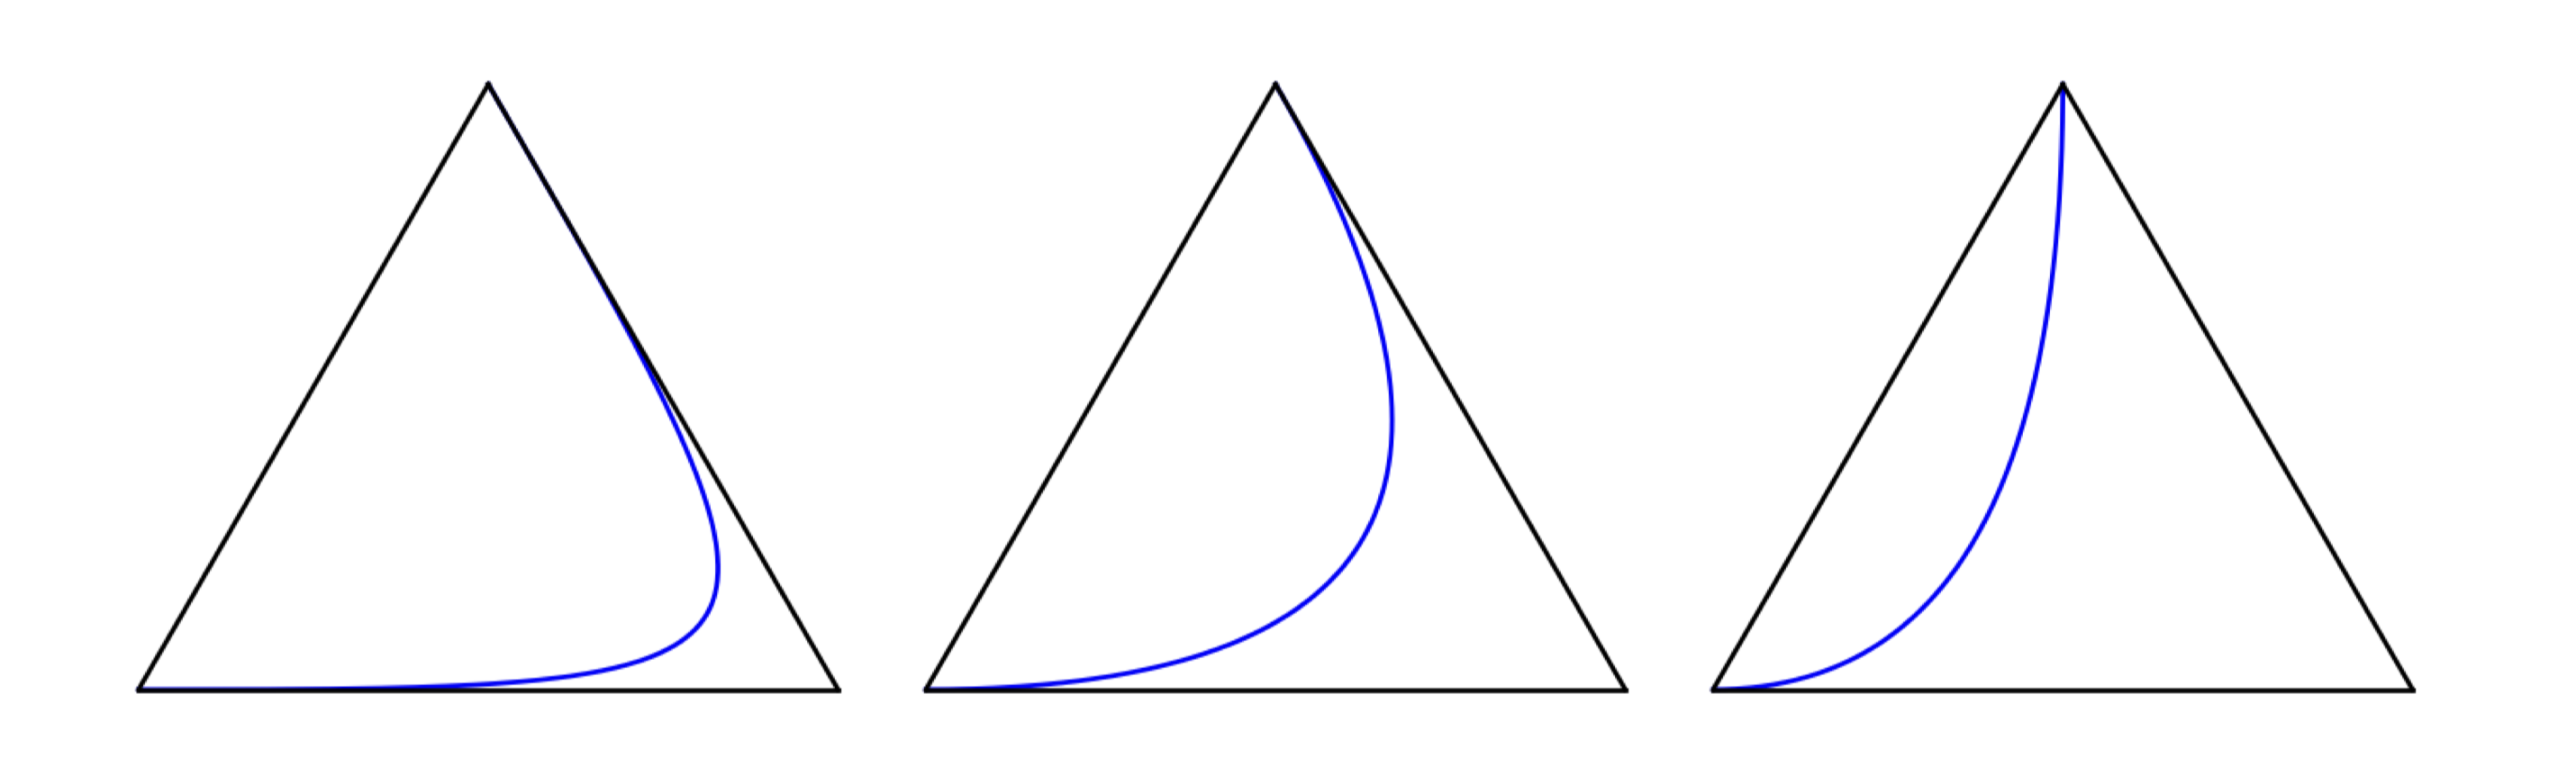
\includegraphics[width=0.8\textwidth]{assets/fundamental-models-delta-2.png}
    \caption{From left to right, the illustration depicts the models parametrized \( ((1-\theta)^3, 3\theta(1-\theta), \theta^3) \), \( ((1-\theta)^2, 2\theta(1-\theta), \theta^2) \), \( (1-\theta, \theta(1-\theta), \theta^2) \), and \( ((1-\theta)^2, \theta, \theta(1-\theta)) \).}

    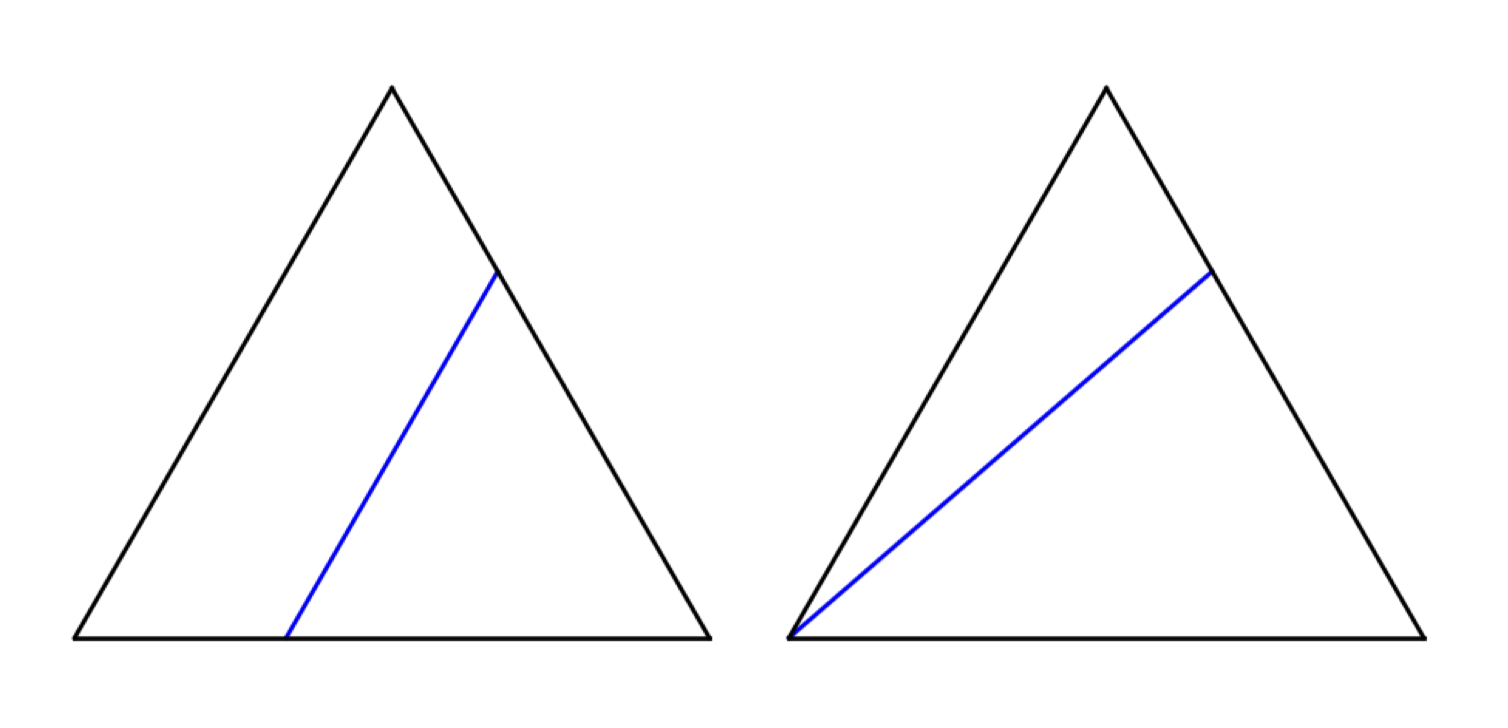
\includegraphics[width=0.55\textwidth]{assets/non-red-models-delta-2.png}
    \caption{This illustration depicts two non-reduced models in \( \Delta_2 \) for \( \lambda = \frac{1}{3} \). They are parametrized by \( \theta \mapsto (\frac{2}{3}\theta, \frac{1}{3}, \frac{2}{3}(1 - \theta)) \) and \( \theta \mapsto (1-\theta, \frac{1}{3}\theta, \frac{2}{3}\theta) \). All other non-reduced models can be obtained by varying \( \lambda \).} 
\end{figure}

We just computed all fundamental models of degree three or less in \( \Delta_2 \). We will see shortly that these are all models in the probability simplex \( \Delta_2 \). Of course, \( \Delta_2 \) contains non-reduced models, too. These are models that come from linear embeddings \( \Psi_{\lambda,k} \) and \( \Psi_{\lambda,k,h} \), see Proposition \ref{prop:linear-embedding-1} and Proposition \ref{prop:linear-embedding-2}. There are infinitely many of them, and for \( \lambda = \frac{1}{3} \) we obtain the models \( \theta \mapsto (\frac{2}{3}\theta, \frac{1}{3}, \frac{2}{3}(1 - \theta)) \) and \( \theta \mapsto (1-\theta, \frac{1}{3}\theta, \frac{2}{3}\theta) \).
\end{example}

\begin{theorem}\label{thm:classification-jekns}
    Every one-dimensional discrete statistical model with rational MLE in \( \Delta_n \) is the image of a reduced model in \( \Delta_m \) under a linear embedding \( \Delta_m \to \Delta_n \) for some \( m \leq n \).

    Moreover, every reduced model \( \mathcal{M} \subset \Delta \) can be written as a composite of finitely many fundamental models \( \mathcal{M} = \mathcal{M}_1 *_{\mu_1} ( \dots *_{\mu_{m-2}}( \mathcal{M}_{m-1} *_{\mu_{m-1}} \mathcal{M}_m) ) \)
    for some \( m < n \) and \( \mu_1, \dots, \mu_m \in (0,1) \).
\end{theorem}

\begin{proof}
    See Proposition \ref{prop:composition-fundamental}, Proposition \ref{prop:linear-embedding-1}, and Proposition \ref{prop:linear-embedding-2}.
\end{proof}

\section{On the Finiteness of Fundamental Models}

After establishing that fundamental models serve as the building blocks for all models, we will prove that for \( n \leq 4 \), there are only finitely many fundamental models in \( \Delta_n \). This result was first established by Bik and Marigliano, and we adopt their approach. To begin, we present the following proposition.

\begin{theorem}\label{thm:degree-fundamental-models}
    Let \( \mathcal{M} \) be a one-dimensional discrete statistical model with rational MLE in \( \Delta_n \). For \(n \leq 4 \), we have \( \mathrm{deg}(\mathcal{M}) \leq 2n - 1\).
\end{theorem}

Given this theorem, it is easy to show the finiteness of fundamental models.

\begin{theorem}\label{thm:finiteness-fundamental-models}
    There are only finitely many fundamental models in \( \Delta_n \) for all \( n \leq 4 \).
\end{theorem}

\begin{proof}
    Let \( n \leq 4 \).
    By Theorem \ref{thm:degree-fundamental-models}, we know that the degree of a fundamental model is at most \( 2n - 1 \). Since the number of supports of a fundamental model of degree \( 2n - 1 \) is finite, there are only finitely many fundamental models in \( \Delta_n \).
\end{proof}

It turns out that proving Theorem \ref{thm:degree-fundamental-models} only for fundamental models is sufficient.

\begin{theorem}\label{thm:degree-fundamental-models-reduced}    
    Let \( N \in \mathbb{N} \). If the upper bound \( \mathrm{deg}(\mathcal{M}) \leq 2n - 1 \) holds for all \( n \leq N \) and for all fundamental models \( \mathcal{M} \in \Delta_n \), then this upper bound also holds for all statistical models, including non-fundamental ones, in \( \Delta_n \) for all \( n \leq N \).
\end{theorem}

\begin{proof}
    Let $N \in \mathbb{N}$ and $n \leq N$.
    Assume there is some non-fundamental model $\mathcal{M}'$ in $\Delta_n$ of degree greater than $2n - 1$. By Corollary \ref{cor:fundamental-models-ksmlkdf} there exists a fundamental model $\mathcal{M}$ in $\Delta_m$ for some $m < n$ of degree greater than $2m - 1$. This contradicts the assumption that the degree of fundamental models is at most $2n' - 1$ for all $n' \leq N$.
\end{proof}

This justifies that our north star is to prove the following theorem.

\begin{theorem}\label{thm:degree-fundamental-models-fundamental}
    Let \( \mathcal{M} \) be a fundamental model in \( \Delta_n \). For \(n \leq 4 \), we have \( \mathrm{deg}(\mathcal{M}) \leq 2n - 1\).
\end{theorem}

The first step is introducing a combinatorial puzzle to count fundamental models using the sequence \((w_k, i_k, j_k)_{k=0}^{n}\), which characterizes these models. 
\chapter{Chipsplitting Games}

The notion of a chipsplitting game was introduced by \cite{bik2022classifying} as a combinatorial approach to classifying one-dimensional discrete statistical models with rational maximum likelihood estimator. It was inspired by \emph{chipfiring games} and for a subset of chipfiring games, the chipsplitting game is equivalent to the chipfiring game. We refer to \cite{klivans2018mathematics} for a comprehensive introduction to chipfiring games. 

\section{Basic Definitions}

Let us define the notion of a chipsplitting game.

\begin{definition}
    Let $(V,E)$ be a directed graph without loops.

    \begin{enumerate}
        \item A \emph{chip configuration} is a vector \( \mathbf{w} = (w_v)_{v \in V} \in \mathbb{Z}^{V} \) such that there are only finitely many nonzero components \( w_k \).
        \item The \emph{initial configuration} is the chip configuration \( \mathbf 0 \in \mathbb{Z}^V \).
        \item A \emph{splitting move} at \( u \in V \) maps a chip configuration \( \mathbf w \) to some chip configuration \( \mathbf{w}' \) defined by 
        \begin{align*}
            w'_v \coloneqq \begin{cases}
                w_v -1 & \text{if } v = u, \\
                w_v + 1 & \text{if } (u,v) \in E \\
                w_v & \text{otherwise}.
            \end{cases}
        \end{align*}
        This map is denoted by \( \mathrm{split}_u \).
        \item An \emph{unsplitting move} at \( u \in V \) maps \( \mathbf w' \) back to \( \mathbf{w} \). This map is denoted by \( \mathrm{unsplit}_u \).
        \item A \emph{chipsplitting game} is a finite sequence of splitting and unsplitting moves.
        \item An \emph{outcome of a chipsplitting game} is the chip configuration obtained from applying the sequence of splitting and unsplitting moves defined by the game at the initial configuration.
        \item Any outcome of a chipsplitting game is called an \emph{outcome}.
    \end{enumerate}
\end{definition}

\begin{proposition}\label{prop:commutativity}
    The order of the moves in a chipsplitting game does not affect the outcome.
\end{proposition}

\begin{proof}
    This follows from commutativity of addition.
\end{proof}

Note that all moves are reversible. Thus, we obtain the following corollary with Proposition \ref{prop:commutativity}.

\begin{corollary}
    Let \( \mathbf{w} \) be an outcome. Then, there exists a chipsplitting game whose outcome is \( \mathbf{w} \) and where at no point both a splitting and an unsplitting move are applied at the same vertex.
\end{corollary}

Games that satisfy the condition in the corollary are called \emph{reduced}. We will only consider reduced games in this thesis for simplicity. The map 
\begin{align*}
    \left\{ \text{reduced games on \( (V,E) \)} \right\} / \sim \quad &\to \quad  \left\{ g: V' \to \mathbb{Z} : \# \{ p \in V' : g(p) \neq 0 \} < \infty \right\} \\
    f &\mapsto (p \mapsto \text{number of moves at \( p \) in game \( f \)})
\end{align*}
is a bijection, where \( V' \subset V \) is the subset of vertices with at least one outgoing edge. The equivalence relation \( \sim \) is defined by \( f \sim g \) if \( f \) and \( g \) are the same up to reordering. Unsplitting moves are counted negatively by \( p \mapsto \text{number of moves at \( p \) in game \( f \)} \). Using the map above we identify a chipsplitting game with its corresponding function \( V' \to \mathbb{Z} \). For every outcome \( \mathbf{w} = (w_v)_{v \in V} \) we have 
\begin{align*}
    w_v = -f(v) + \sum_{u\in V', (u,v) \in E} f(u),
\end{align*}
where we define \( f(v) = 0 \) for \( v \notin V \).

Now, we define the directed graphs that we will consider in this thesis. For \( d \in \mathbb{N} \cup \left\{ \infty \right\} \) we write 
\begin{align*}
    V_d &\coloneqq \left\{ (i,j) \in \mathbb{Z}^2_{\geq 0} \mid i+j \leq d \right\},\\
    E_d &\coloneqq \left\{ (v,v+e) \mid v \in V_{d-1}, e \in \left\{ (1,0), (0,1) \right\} \right\}.
\end{align*}

\begin{definition}
    The degree \( \mathrm{deg}(\mathbf{v}) \) of a vertex \( \mathbf{v} = (i,j) \) is defined as \( i + j \).
\end{definition}

\begin{example}
    A chip configuration \( \mathbf{w} = (w_{i,j})_{(i,j) \in V_d} \in \mathbb{Z}^{V_d} \) can be illustrated as a triangle of numbers where \( w_{i,j} \) is placed at the position \( (i,j) \) in the triangle. For example, \( w_{2,4} = 4 \) means that the value \( 4 \) is placed in the second column and fourth row of the triangle. The following is an example of a sequence of chip configurations for \( d = 3 \):
    \begin{verbatim}
.            .            .            1            1            1
. .          . .          1 .          . 1          . 1          . .
. . .        1 . .        . 2 .        . 2 .        . 2 1        . 3 .
0 . . .     -1 1 . .     -1 . 1 .     -1 . 1 .     -1 . . 1     -1 . . 1
    \end{verbatim}
    When \( w_{i,j} = 0 \), we omit the value in the triangle and write a dot instead. The sequence above starts with the initial configuration and then applies a splitting move at the vertex \( (0,0), (1,0), (0,1), (0,2) \) and \( (2,0) \). Finally, we apply an unsplitting move at the vertex \( (1,1) \) to obtain the final configuration. Coming back to figure \ref{fig:binom-discrete-model-visual}, we see that it is represented as the third configuration of the triangle above.
\end{example}

Let us define some more terminology.

\begin{definition}
    Let \( \mathbf{w} = (w_{i,j})_{(i,j) \in V_d} \) be a chip configuration.
    \begin{enumerate}
        \item The \emph{positive support} of \( \mathbf{w} \) is defined as \( \mathrm{supp}^+(\mathbf{w}) \coloneqq \left\{ (i,j) \in V_d\mid w_{i,j} > 0 \right\} \).
        \item The \emph{negative support} of \( \mathbf{w} \) is defined as \( \mathrm{supp}^-(\mathbf{w}) \coloneqq \left\{ (i,j) \in V_d\mid w_{i,j} < 0 \right\} \).
        \item The \emph{support} of \( \mathbf{w} \) is defined as the union of the positive and negative support.
        \item The \emph{degree} of \( \mathbf{w} \) is defined as \( \mathrm{deg}(\mathbf{w}) \coloneqq \mathrm{max}\left\{ i+j \mid (i,j) \in \mathrm{supp}(\mathbf{w}) \right\} \).
        \item We say \( \mathbf{w} \) is \emph{valid} if its negative support is empty or only contains \( (0,0) \).
    \end{enumerate}
\end{definition}

We are interested in \emph{outcomes} that are \emph{valid} since they will correspond to reduced models as we will see later. For that reason, it would be convenient to have a criterion for when a chip configuration is an outcome. The next section will provide such a criterion with the help of \emph{Pascal equations}.

\begin{example}\label{ex:dknfkdjsfnsdj}
    Consider the following chip configuration:
    \begin{verbatim}
        · 
        ·   1 
        1   ·   5 
        ·   5   ·   2 
        1   .   .   5   . 
        ·   .   8   .   .   2 
       -2   ·   .   .   .   2   . 
    \end{verbatim}
    We clearly see that this configuration is valid, but is it also an outcome of a chipsplitting game? Currently, the only way to answer this question is to apply all possible sequences of splitting and unsplitting moves to the initial configuration and check if the outcome is the given configuration. In the next section, we present an easily computable characterization to answer this question.
\end{example}


%TO-DO: define weakly valid if we havent done so

\section{Pascal Equations}

In this chapter we will establish that outcomes are roots of Pascal equations. So let us first define Pascal equations which are special cases of \emph{linear forms}.

\begin{definition}
    A \emph{linear form} on \( \mathbb{Z}^{V_d} \) is a map of the form
    \begin{align*}
        \mathbb{Z}^{V_d} \to \mathbb{Z}, \quad \mathbf{w} \mapsto \sum_{(i,j) \in V_d} c_{i,j} w_{i,j}.
    \end{align*}
    It is denoted by \( \sum_{(i,j) \in V_d} c_{i,j} x_{i,j} \).
\end{definition}

\begin{definition}
    A \emph{Pascal form} on \( \mathbb{Z}^{V_d} \) is a linear form \( \sum_{(i,j) \in V_d} c_{i,j} x_{i,j} \) on \( \mathbb{Z}^{V_d} \) satisfying 
    \begin{align*}
        c_{i,j} = c_{i+1,j} + c_{i,j+1} \quad \text{for all } (i,j) \in V_{d-1}.
    \end{align*}
\end{definition}

\begin{example}
    We can visualize a Pascal form as a triangle of numbers where \( c_{i,j} \) is placed at the position \( (i,j) \) in the triangle. Here are examples of Pascal forms for \( d = 2 \):
    \begin{verbatim}
  0               1               0               0
  1  1            1  0            0  0            1  1
  2  1  0         1  0  0         1  1  1         0 -1 -2
    \end{verbatim}
\end{example}

Evaluating Pascal equations is invariant under splitting and unsplitting moves. 

\begin{proposition}\label{prop:pascal-invariance}
    Let \( \mathbf{w}\in \mathbb{Z}^{V_d} \) be a chip configuration. Let \( p = \sum c_{i,j}x_{i,j} \) be a Pascal equation on \( \mathbb{Z}^{V_d} \). Then,  we have \( p(\mathbf w) = p(\mathrm{split}_u(\mathbf w)) = p(\mathrm{unsplit}_{v}(\mathbf w)) \) for all \( u, v \in V_{d-1} \).
\end{proposition}

\begin{proof}
    Let \( u \coloneqq (i',j') \in V_{d-1} \).
    By the Pascal property, we have 
    \begin{align*}
        c_{i'+1,j'} + c_{i',j'+1} - c_{i',j'}= 0.
    \end{align*}
    Thus, we have 
    \begin{align*}
        p(\mathrm{split}_u(\mathbf w)) &= \sum_{(i,j) \in V_d} c_{i,j} (\mathrm{split}_u(\mathbf w))_{i,j} \\
        &= \sum_{(i,j) \in V_d} c_{i,j} \begin{cases}
            w_{i,j} - 1 & \text{if } (i,j) = u, \\
            w_{i,j} + 1 & \text{if } (i,j) \in \left\{ (i'+1,j'), (i',j'+1) \right\} \\
            w_{i,j} & \text{otherwise}
        \end{cases}\\&= \sum_{(i,j) \in V_d} c_{i,j} w_{i,j} = p(\mathbf w).
    \end{align*}
    Similarly, we can show that \( p(\mathrm{unsplit}_v(\mathbf w)) = p(\mathbf w) \) for all \( v \in V_{d-1} \).
\end{proof}

\begin{corollary}
    Let \( \mathbf{w}\in \mathbb{Z}^{V_d} \) be an outcome. Let \( p = \sum c_{i,j}x_{i,j} \) be a Pascal equation on \( \mathbb{Z}^{V_d} \). Then, \( p(\mathbf w) = 0 \).
\end{corollary}

\begin{proof}
    Clearly, we have \( p(\mathbf 0) = 0 \). Then, we use Proposition \ref{prop:pascal-invariance} and the fact that \( \mathbf{w} \) is obtained from the initial configuration \( \mathbf{0} \) by a sequence of splitting and unsplitting moves.
\end{proof}

This demonstrates that outcomes are roots of Pascal equations. The converse is also true as we will see now. This is one of the most important results; so let us state it now.

\begin{theorem}\label{thm:pascal-outcome}
    Let \( \mathbf{w}\in \mathbb{Z}^{V_d} \) be a chip configuration. Then, \( \mathbf{w} \) is an outcome if and only if \( \mathbf{w} \) is a root of all Pascal equations on \( \mathbb{Z}^{V_d} \).
\end{theorem}

The direction left to right is the content of the previous corollary. For the other direction life would be easier if we had not to deal with infinitely many Pascal equations. So let us fix this first by introducing a basis from which we can generate all Pascal equations through linear combinations.

\begin{example}\label{ex:pascal-basis}
    Fix the degree \( d = 2 \). We later claim that the following set of Pascal forms is a basis:
    \begin{verbatim}
        0               0               1               
        0  0            1  1            0 -1           
        1  1  1,        0 -1 -2,        0  0  1.     
    \end{verbatim}
    Note that the first column of each Pascal form is a unit vector in \( \mathbb{R}^3 \). We can also fix the first row of each Pascal form to be a unit vector in \( \mathbb{R}^3 \):
    \begin{verbatim}
        1              -2               1               
        1  0           -1  1            0 -1           
        1  0  0,        0  1  0,        0  0  1.
    \end{verbatim} 
    We will denote the first set of Pascal forms by \( \left\{ \mathrm{col}(0), \mathrm{col}(1), \mathrm{col}(2) \right\} \) and the second set by \( \{ \mathrm{row}(0), \mathrm{row}(1), \mathrm{row}(2) \} \).
\end{example}

To generalize the example above to an arbitrary degree \( d \in \mathbb{N} \) and to vectors beyond unit vectors, we assert that there exists a unique Pascal form whose first column is any chosen vector.

\begin{proposition}\label{prop:supsup-pascal}
    Let \( \mathbf{a} = (a_0, \dots, a_d) \) be any vector with integer entries. Then, the following two statements hold:
    \begin{enumerate}
        \item There exists a unique Pascal form \( \sum c_{i,j}x_{i,j} \) such that \( c_{0,\cdot} = \mathbf a \).
        \item There exists a unique Pascal form \( \sum c_{i,j}x_{i,j} \) such that \( c_{\cdot,0} = \mathbf a \).
    \end{enumerate}
\end{proposition}

\begin{proof}
    Set \( c_{0,\cdot} \coloneqq \mathbf a \). Define \( c_{i+1,j} \coloneqq c_{i,j} - c_{i,j+1}\) for all \( (i,j) \in V_d \) with \( i=0 \). Then, we use the same formula to define \( c_{i+1,j} \) for all \( (i,j) \in V_d \) with \( i=1 \). We repeat this process until we have defined all \( c_{i,j} \) for \( (i,j) \in V_d \).

    For the second statement, we set \( c_{\cdot,0} \coloneqq \mathbf a \). Define \( c_{i,j+1} \coloneqq c_{i,j} - c_{i+1,j}\) for all \( (i,j) \in V_d \) with \( j=0 \). Then, we use the same formula to define \( c_{i,j+1} \) for all \( (i,j) \in V_d \) with \( j=1 \). We repeat this process until we have defined all \( c_{i,j} \) for \( (i,j) \in V_d \).
\end{proof}

Let us define our first two Pascal form bases.

\begin{definition}
    Let \( k = 0, \dots, d \) and \( \mathbf e_k \in \mathbb{R}^{d+1} \) be the \( k \)-th unit vector. 
    \begin{itemize}
        \item We define \( \mathrm{col}(k) \) to be the unique Pascal form \( \sum c_{i,j}x_{i,j} \) such that \( c_{0,\cdot} = \mathbf e_k \).
        \item We define \( \mathrm{row}(k) \) to be the unique Pascal form \( \sum c_{i,j}x_{i,j} \) such that \( c_{\cdot,0} = \mathbf e_k \).
    \end{itemize}
\end{definition}

For examples of the Pascal forms \( \mathrm{col}(k) \) and \( \mathrm{row}(k) \) for \( d = 2 \) see Example \ref{ex:pascal-basis}. We provide another example for \( d = 7 \).

\begin{example}
    Let us consider the Pascal form \( \mathrm{col}(3) \) for \( d = 7 \). We visualize this Pascal form as follows: 
    \begin{verbatim}
        · 
        ·   · 
        ·   ·   · 
        ·   ·   ·   · 
        1   1   1   1   1 
        ·  -1  -2  -3  -4  -5 
        ·   ·   1   3   6  10  15 
        ·   ·   ·  -1  -4 -10 -20 -35.
    \end{verbatim}

    The Pascal form \( \mathrm{row}(3) \) is visualized as follows:
    \begin{verbatim}
        -35 
        -20  15 
        -10  10  -4 
        -4   6  -4   1 
        -1   3  -3   1   . 
         ·   1  -2   1   .   . 
         ·   ·  -1   1   .   .   . 
         ·   ·   ·   1   .   .   .   .
    \end{verbatim}
\end{example}

\begin{proposition}\label{prop:pascal-formulas}
    For all integers \( k = 0, \dots, d \) the following formulas hold:
    \begin{align*}
        \mathrm{col}(k)  &= (-1)^k \sum_{(i,j) \in V_d} (-1)^j \binom{i}{k-j} x_{i,j}, \\
        \mathrm{row}(k) &= (-1)^k \sum_{(i,j) \in V_d} (-1)^i \binom{j}{k-i} x_{i,j}.
    \end{align*} 
    Note that \( \binom{a}{b} = 0 \) for \( b < 0 \) or \( b > a \).
\end{proposition}

\begin{proof}
    We claim that \( (-1)^k \sum_{(i,j) \in V_d} (-1)^j \binom{i}{k-j} x_{i,j} \) is a Pascal equation. To see that observe 
    \begin{align*}
        (-1)^j \binom{i+1}{k-j} + (-1)^{j+1} \binom{i}{k-j-1} &= (-1)^j \binom{i}{k-j}
    \end{align*}
    for all \( (i,j) \in V_{d} \) due to \(  \binom{a}{b+1} + \binom{a}{b} = \binom{a+1}{b+1} \) where we set \( a = i \) and \( b = k-j-1 \). Next, we see that \( (-1)^{k+j} \binom{0}{k-j} = \delta_{jk} \). Thus, \( (-1)^k \sum_{(i,j) \in V_d} (-1)^j \binom{i}{k-j} x_{i,j} \) is indeed \( \mathrm{col}(k) \).

    By symmetry of the binomial coefficients, we can use the same argument to show the second formula.
\end{proof}

We now show that \( \left\{ \mathrm{col}(k) \right\}_{k=0}^{d} \) is indeed a basis for all Pascal forms on \( \mathbb{Z}^{V_d} \).

\begin{proposition}\label{prop:pascal-basis}
    Let \( p \) be a Pascal form on \( \mathbb Z^{V_d} \). The following statements hold:
    \begin{enumerate}
        \item There exist unique coefficients \( \mu_0, \dots, \mu_d \in \mathbb{Z} \) such that 
        \( p = \mu_0 \mathrm{col}(0) + \dots + \mu_d \mathrm{col}(d) \).

        \item There exist unique coefficients \( \lambda_0, \dots, \lambda_d \in \mathbb{Z} \) such that 
        \( p = \mu_0 \mathrm{row}(0) + \dots + \mu_d \mathrm{row}(d) \).
    \end{enumerate}
\end{proposition}

\begin{proof}
    Let \( p = \sum c_{i,j}x_{i,j}\) be a Pascal form on \( \mathbb{Z}^{V_d} \). If we try to solve the equation
    \begin{align}\label{eq:234324324}
        \sum_{(i,j) \in V_d} c_{i,j}x_{i,j} = \lambda_0 \mathrm{col}(0) + \dots + \lambda_d \mathrm{col}(d)
    \end{align}
    for \( \lambda_0, \dots, \lambda_d \), then due to Proposition \ref{prop:pascal-formulas} we see for all \( (i,j)\in V_d \) that we have
    \begin{align*}
        c_{i,j} &= \lambda_0 (-1)^{0+j} \binom{i}{0-j} + \lambda_1 (-1)^{1+j} \binom{i}{1-j} + \dots + \lambda_d (-1)^{d+j} \binom{i}{d-j} \\
        &= \lambda_j (-1)^{2j} \binom{i}{0} + \lambda_{j+1} (-1)^{2j+1} \binom{i}{1} + \dots + \lambda_{i+j} (-1)^{2j+i} \binom{i}{i}.
    \end{align*}
    We see \(c_{0, \cdot} = (\lambda_0, \cdots, \lambda_d) \). Thus we set the coefficients \( \boldsymbol \mu \coloneqq c_{0, \cdot} \) and by Proposition \ref{prop:supsup-pascal} we see that \( \sum_{(i,j) \in V_d} c_{i,j}x_{i,j} = \mu_0 \mathrm{col}(0) + \dots + \mu_d \mathrm{col}(d) \). Moreover, the same proposition shows that the coefficients \( \lambda_0, \dots, \lambda_d \) in Equation \ref{eq:234324324} are uniquely determined. 
    
    For the second statement we use the same argument.
\end{proof}

\begin{corollary}\label{cor:pascal-basis-2323}
    The set \( \left\{ \mathrm{col}(k) \right\}_{k=0}^d \) is a basis for all Pascal forms on \( \mathbb{Z}^{V_d} \). The same holds for \( \left\{ \mathrm{row}(k) \right\}_{k=0}^d \). 
\end{corollary}

\begin{proof}
    This follows from the previous proposition.
\end{proof}

Let us come back to Theorem \ref{thm:pascal-outcome}. We can now prove the other direction; namely that roots of all Pascal equations on \( \mathbb{Z}^{V_d} \) are outcomes.

\begin{proposition}\label{thm:pascal-outcome-converse}
    Let \( \mathbf{w}\in \mathbb{Z}^{V_d} \) be a chip configuration. If for all Pascal equations \( p \) on \( \mathbb{Z}^{V_d} \) we have \( p(\mathbf w) = 0 \), then \( \mathbf{w} \) is an outcome.
\end{proposition}

\begin{proof}
    Let \( \mathbf{w}\in \mathbb{Z}^{V_d} \) be a chip configuration.
    By assumption
    \begin{align}\label{eq:324324234324324}
        \mathrm{col}(\mathrm{deg}(\mathbf w))(\mathbf w) = 0.
    \end{align}
    Note that by Proposition \ref{prop:pascal-formulas} for \( \mathrm{col}(\mathrm{deg}(\mathbf w)) = \sum c_{i,j} x_{i,j}\) we have \( c_{i,\mathrm{deg}(\mathbf w) - i} = (-1)^{i} \) for all \( i =0, \dots, \mathrm{deg}(\mathbf w) \). Moreover, we have 
    \begin{align}\label{eq:34kl}
        c_{i,j} = 0 \quad \text{for all \( i+j < \mathrm{deg}(\mathbf w) \)}
    \end{align}
     by Proposition \ref{prop:pascal-formulas}. Together with Equation \ref{eq:324324234324324} and \ref{eq:34kl} we obtain 
    \begin{align}\label{eq:2j2j1kjkj}
        \sum_{i=0}^{\mathrm{deg}(\mathbf w)}(-1)^i w_{i, \mathrm{deg}(\mathbf w) - i} = 0.
    \end{align}
    Furthermore, we know that there exists a unique minimal set of splitting or unsplitting moves at vertices \( (i,j) \) of degree \( \mathrm{deg}(\mathbf w) - 1 \) such that applied to \( \mathbf w \) we obtain a chip configuration \( \mathbf w' \) with \( w'_{i,j} = 0 \) for all \( i =0, ... , \mathrm{deg}(\mathbf w) \). We call applying these set of moves to \( \mathbf w \) \emph{retraction}.
    
    \begin{verbatim}
        .
        .   .
        .   .   .
        *   .   .   .
        *   *   .   .   .
        *   *   *   .   .   .
        *   *   *   *   .   .   .
        *   *   *   *   *   .   .   .
        *   *   *   *   *   *   .   .   .
            |
            |
            | retraction of w of degree five
            |
            |
            V
        .
        .   .
        .   .   .
        .   .   .   .
        *   .   .   .   .
        *   *   .   .   .   .
        *   *   *   .   .   .   .
        *   *   *   *   .   .   .   .
        *   *   *   *   *   .   .   .   .
    \end{verbatim}
    Thus, \( \mathbf w' \) has degree less than \( \mathrm{deg}(\mathbf w) \).
    By Proposition \ref{prop:pascal-invariance} \( \mathbf w' \) is also a root of all Pascal equations. We repeat the retraction process \( \mathrm{deg}(\mathbf w) \) many times until we obtain some chip configuration of degree \( 0 \). This chip configuration is the initial configuration due to Equation \ref{eq:2j2j1kjkj}. Thus, \( \mathbf w \) is an outcome.
\end{proof}

We have shown Theorem \ref{thm:pascal-outcome}. Characterizing outcomes as roots of Pascal equations is a powerful tool to determine if a chip configuration is an outcome.

\begin{algorithm}
\caption{Validating outcomes}\label{alg:pascal-equation-outcome}
    \begin{algorithmic}[1]
    \Require chipsplitting configuration \( \mathbf w \in \mathbb{Z}^{V_d} \)
    \Ensure \texttt{True} if \( \mathbf w \) is an outcome, \texttt{False} otherwise

    \Function{isOutcome}{$A, n$}
    \State initialize set \( S = \left\{ \mathrm{col}(0), \dots, \mathrm{col}(\mathrm{deg}(\mathbf w)) \right\} \)
    \For{$p$ of $S$}
        \If{$p(\mathbf w) \neq 0$} 
        \State \Return \texttt{False}
        \EndIf
    \EndFor
    \State \Return \texttt{True}
    \EndFunction
    \end{algorithmic}  
\end{algorithm}

\begin{proof}[Proof of correctness of Algorithm \ref{alg:pascal-equation-outcome}]
    This follows from Theorem \ref{thm:pascal-outcome}.
\end{proof}

\begin{example}
    Returning to Example \ref{ex:dknfkdjsfnsdj}, we see that the chip configuration is a root of all Pascal equations \( \mathrm{col}(0), \dots, \mathrm{col}(6) \) using Algorithm \ref{alg:pascal-equation-outcome}. Thus, the chip configuration is an outcome.
\end{example}

\section{Valid Outcomes and Reduced Statistical Models}

In the previous sections, we have established that outcomes are roots of Pascal forms. Now, we will demonstrate that a subset of \emph{valid outcomes} are in one-to-one correspondence with reduced statistical models. Thus, we obtain not only a combinatorial characterization of reduced statistical models through chip-splitting games but also an algebraic characterization through Pascal equations. As before, statistical models mean one-dimensional discrete statistical models with rational maximum likelihood estimator.

We remind that valid chipsplitting configurations are those where the negative support is empty or only contains the vertex \( (0,0) \). Hence, valid outcomes are roots of Pascal equations whose negative supports are empty or only contain the vertex \( (0,0) \). 

The function \( \mathbf w(\mathcal{M}) \) maps reduced models \( \mathcal{M} = (w_k, i_k, j_k)^{n}_{k=0} \) to chip configurations \( \mathbf w(\mathcal{M}) = (w_{i,j})_{(i,j) \in V_\infty} \) by 
\begin{align*}
    w_{i,j} \coloneqq \begin{cases}
        -1 & \text{if } (i,j) = (0,0), \\
        w_k & \text{if } (i,j) = (i_k, j_k) \text{ for some } k, \\
        0 & \text{otherwise}.
    \end{cases}
\end{align*}

Note that the map \( \mathbf w(\mathcal{M}) \) defines a \emph{real} chipsplitting games; the rules of the game are the same as for integer chipsplitting games.

\begin{example}\label{ex:binomial-model-chip-three}
    The binomial model \( ((1,3,0), (3,2,1), (3,1,2), (1,0,3)) \) with three trials is mapped to the chip configuration below:
    \begin{verbatim}
        1
        ·   3  
        .   ·   3
       -1   .   .   1.
    \end{verbatim}
\end{example}

\begin{example}\label{ex:alpaca-andy}
    Does the following valid real outcome from Example \ref{ex:dknfkdjsfnsdj} induce a reduced statistical model through the inverse map \( \mathbf w^{-1} \)?
    \begin{verbatim}
        · 
        ·   0.5 
      0.5     ·   2.5 
        ·   2.5     ·     1 
      0.5     .     .   2.5     . 
        ·     .     4     .     .     1 
       -1     ·     .     .     .     1     . 
    \end{verbatim} 
    The outcome would correspond to the reduced model
    \begin{gather*}
        \mathcal{M} = ((0.5, 2, 0), (0.5, 4, 0), (2.5, 1,3), (0.5, 1, 5), (4, 2,1), (2.5, 2, 4),\\ (2.5, 3,2), (1, 3,3), (1, 5,0), (1,5,1))
    \end{gather*}
    in the probability simplex \( \Delta_9 \). As it turns out \( \mathcal{M} \) is indeed a reduced statistical model by the next theorem.
\end{example}

\begin{theorem}\label{thm:outcome-reduced-model}
    The map \( \mathcal{M} \mapsto w(\mathcal{M}) \) is a bijection between reduced statistical models and valid real outcomes \( \mathbf w \in \mathbb{R}^{V_\infty} \) with \( w_{0,0} = -1 \).
\end{theorem}

\begin{figure}[H]
    \centering
    % https://tikzcd.yichuanshen.de/#N4Igdg9gJgpgziAXAbVABwnAlgFyxMJZABgBpiBdUkANwEMAbAVxiRAB12cYAPHYAE4woTAMbCABAFtoMBnAC+IBaXSZc+QigDM5KrUYs2nbn2D0GWKBIhMcoiFPhKF+4QHN4RUADMBjpABGahwIJDIQAAsYOig2HAB3CGjYhBC6LAY2SIgIAGtGHGUKBSA
\begin{tikzcd}
    \text{reduced models} &  &  & \text{valid outcomes} \arrow[lll, two heads, hook']
    \end{tikzcd}
    \caption{Bijection between reduced models and valid real outcomes \( \mathbf w \) with \( w_{0,0} = -1 \)}
\end{figure}


To show this theorem, we need to do some preparations. Let \( \mathbb{R}[\theta]_{\leq d} \) denote the vector space of polynomials in the variable \( \theta \) of degree at most \( d \) with real coefficients. Similarly, we define \( \mathbb{Z}[\theta]_{\leq d} \) and \( \mathbb{Q}[\theta]_{\leq d} \). Next, we introduce the linear map \( \alpha_{d}^{\mathbb R} \) that maps real chip configurations to real polynomials:
\begin{align*}
    \alpha_d^{\mathbb R}: \mathbb{R}^{V_d} &\to \mathbb{R}[\theta]_{\leq d}, \\
    \mathbf{w} &\mapsto \sum_{(i,j) \in V_d} w_{i,j} \theta^{i}(1-\theta)^j.
\end{align*}
We define the map \( \alpha_d^{\mathbb Z} \) and \( \alpha_d^{\mathbb Q} \) for integer and rational chip configurations analogously.

\begin{lemma}\label{lem:kernel-noo}
    The following statements hold true for all \( d \in \mathbb{N} \cup \left\{ \infty \right\} \):
    \begin{enumerate}
        \item \( \left\{ \mathbf w \in \mathbb R^{V_d} \mid \text{\( \mathbf{w} \) is an outcome} \right\} = \mathrm{kernel}(\alpha_d^{\mathbb R})\);
        \item \( \left\{ \mathbf w \in \mathbb Z^{V_d} \mid \text{\( \mathbf{w} \) is an outcome} \right\} = \mathrm{kernel}(\alpha_d^{\mathbb Z})\);
        \item \( \left\{ \mathbf w \in \mathbb Q^{V_d} \mid \text{\( \mathbf{w} \) is an outcome} \right\} = \mathrm{kernel}(\alpha_d^{\mathbb Q})\).
    \end{enumerate}
\end{lemma}

\begin{proof}
    We only prove the first statement. The other two statements are proven analogously. Note that it suffices to show the statement for \( d < \infty \) since \( \alpha_\infty^\mathbb{R} \) is the direct limit of \( \alpha^{\mathbb R}_0, \alpha^{\mathbb R}_1, \alpha^{\mathbb R}_2, \dots \), and so on.

    Let \( d < \infty \). By Corollary \ref{cor:pascal-basis-2323}, the codimension of the outcome space is \( d+1 \), as it is defined by the roots of the Pascal forms \( \mathrm{col}(0), \dots, \mathrm{col}(d) \). 

    Let \( f(\theta) = \lambda_0 + \lambda_1 \theta + \dots + \lambda_d \theta^d  \) be a polynomial in \( \mathbb R \) of degree at most \( d \). Define a chipsplitting configuration \( \mathbf{w} \) by 
        \begin{align*}
            w_{i,j} \coloneqq \begin{cases}
                \lambda_i & \text{if } j=0, \\
                0 & \text{otherwise}.
            \end{cases}
        \end{align*}
    Then, \( \alpha^\mathbb{R}_d(\mathbf w) = f \), which shows that the map \( \alpha^{\mathbb R}_d \) is surjective. Hence, the kernel of \( \alpha^{\mathbb R}_d \) has codimension \( d+1 \); it has equal codimension as the space of outcomes. 

    Finally, we just need to show that the space of outcomes is contained in the kernel of \( \alpha^{\mathbb R}_d \). Since their codimensions are equal, the two spaces must be equal. Let \( \mathbf{w} \in \mathbb{R}^{V_d} \) be an outcome. The value of \( \alpha^{\mathbb R}_d(\mathbf w) \) remains the same if apply splitting or unsplitting moves at arbitrary vertices \( (i,j) \in V_{d-1} \) because we have 
    \begin{align*}
        -\theta^i(1-\theta)^j + \theta^{i+1}(1-\theta)^j + \theta^i(1-\theta)^{j+1} = \theta^i(1-\theta)^j (-1 + \theta + (1 - \theta)) = 0.
    \end{align*}
    The remaining claim follows from \( \alpha_d^{\mathbb{R}}(\mathbf 0) = 0 \).
\end{proof}

We now show Theorem \ref{thm:outcome-reduced-model}.

\begin{proof}[Proof of Theorem \ref{thm:outcome-reduced-model}]
    Let \( \mathcal{M} = (w_k,i_k,j_k)_{k=0}^n \) be a reduced model. 

    \begin{itemize}
        \item First, we need to show that \( \mathbf w \coloneqq w(\mathcal{M}) \) is an outcome; a-priori we only know that it is some chip configuration. By definition of \( w(\mathcal{M}) \), we have that \( w_{0,0} = -1 \). Since \( \mathcal{M} \) is a statistical model, we know that \( \sum_{k=0}^n w_k \theta^{i_k} (1-\theta)^{j_k} \equiv 1 \). Thus, \( \alpha_d^{\mathbb R}(\mathbf w) = \sum_{k=0}^n w_k \theta^{i_k} (1-\theta)^{j_k} -1 \equiv 0 \). Thus, \( \mathbf{w} \in \mathrm{kernel}(\alpha_d^{\mathbb R}) \). By Lemma \ref{lem:kernel-noo}, the chip configuration \( \mathbf w \) is an outcome.
        
        \item \textbf{Injectivity:} Let \( \mathcal{M} = (w_k,i_k,j_k)^n_{k=0} \) and \( \mathcal{M}' = (w'_k,i'_k,j'_k)^n_{k=0} \) be two distinct models. Then, \( w(\mathcal{M}) \neq w(\mathcal{M}') \) (see Remark \ref{rem:equivalent-models}). 
        
        \item \textbf{Surjectivity:} Let \( \mathbf w \in \mathbb{R}^{V_\infty} \) be a valid real outcome with \( w_{0,0} = -1 \). We define 
        \begin{align*}
            w_k &\coloneqq w_{i_k,j_k} \quad \text{for all } k = 0, \dots, n.
        \end{align*}
        Then, \( \mathcal{M}= (w_k,i_k,j_k)^n_{k=0} \) is a reduced model by Lemma \ref{lem:kernel-noo}. We see that \( w(\mathcal{M}) = \mathbf w \). Hence, \( \mathcal{M} \mapsto w(\mathcal{M}) \) is surjective.
    \end{itemize}
\end{proof}

Next, we collect simple results.

\begin{proposition}
    The following statements hold for all reduced models \( \mathcal{M} \):
    \begin{enumerate}
        \item \( \mathrm{supp}^+(w(\mathcal{M})) = \mathrm{supp}^+(\mathcal{M})\).
        \item The map \( \mathcal{M} \mapsto w(\mathcal{M}) \) is degree-preserving.
        \item The outcome \( w(\mathcal{M}) \) is a rational outcome if and only if all the coefficients of \( \mathcal{M} \) are rational.
    \end{enumerate}
\end{proposition}

\begin{proof}
    All three statements follow directly from definitions.
\end{proof}

\begin{proposition}
    Let \( \mathbf{w} \in \mathbb{Q}^{V_\infty} \) be a valid rational outcome. Then, there exist positive \( \lambda \in \mathbb{Q} \) and integral valid outcome \( \mathbf{z} \in \mathbb{Z}^{V_\infty} \) such that \( \mathbf{w} = \lambda \mathbf{z} \).
\end{proposition}

\begin{proof}
    Let \( \mathbf{w} \) be a valid rational outcome. Its support is finite. Thus, there exist \( \mu \in \mathbb{N} \) such that \( \mu \mathbf w \in \mathbb{Z}^{V_\infty} \). Define \( \lambda \coloneqq \frac{1}{\mu} \) and \( \mathbf{v} \coloneqq \mu \mathbf{w} \). Clearly, \( \alpha^{\mathbb{Z}}_{\mathrm{deg}(\mathbf v)}(\mathbf v) = \mu \alpha^{\mathbb{Q}}_{\mathrm{deg}(\mathbf w)}(\mathbf w) \equiv 0 \). By Lemma \ref{lem:kernel-noo}, \( \mathbf v \) is an outcome. It is valid because \( \mu \mathbf w \) is valid.
\end{proof}

\begin{proposition}
    Let \( \mathbf{w} \in \mathbb{R}^{V_\infty} \) be a valid real outcome. If \( w_{0,0} = 0 \), then \( \mathbf{w} = \mathbf 0 \).
\end{proposition}

\begin{proof}
    By Lemma \ref{lem:kernel-noo}, we have \( \sum w_{i,j}\theta^i (1-\theta)^j \equiv 0 \). By assumption, the negative support is empty. Hence, all the \( w_{i,j} \) are non-negative. We evaluate at \( \theta = \frac{1}{2} \) to conclude that the positive support of \( \mathbf w \) is empty. Hence, \( \mathbf w = 0 \).
\end{proof}

Let us go back to Example \ref{ex:binomial-model-chip-three}.

\begin{example}
   We have seen that the valid real outcome below induces a reduced statistical model by Theorem \ref{thm:outcome-reduced-model}.
   \begin{verbatim}
        1
        ·   3  
        .   ·   3
        -1   .   .   1.
    \end{verbatim}
    The outcome has degree three and positive support size four. Can we find another outcome with the same degree but smaller positive support size? Indeed we can unsplitt at vertex \( (1,1) \) to get
    \begin{verbatim}
        1  
        .   .     
        ·   3   .    
       -1   ·   .   1.   
    \end{verbatim} 
    Can we reduce the positive support size further? As it will turn out, we cannot. The positive support size is minimal for a degree three outcome.
\end{example}

\begin{example}
    Let us fix the positive support size to be three. What is the largest degree of a valid real outcome with positive support size three? We have already found
    \begin{verbatim}
        1  
        .   .     
        ·   3   .    
       -1   ·   .   1.   
    \end{verbatim} 
    However is there an even larger one? Once again, the answer is no: by the following theorem, the degree of a valid real outcome with positive support of size three is at most three.
 \end{example}

\begin{theorem}
    s
\end{theorem}

\printbibliography

% \appendix
% \chapter{More Monticello Candidates}

\end{document}
